
\documentclass[10pt,twocolumn]{article}
\usepackage[a4paper,margin=0.72in]{geometry}
\usepackage{fontspec}
\setmainfont{DejaVu Serif}
\setsansfont{DejaVu Sans}
\setmonofont{DejaVu Sans Mono}
\newfontfamily\arabicfont[Script=Arabic,Scale=1.05]{Amiri}
\newcommand{\textarabic}[1]{{\arabicfont #1}}
\usepackage{url,booktabs,multirow,graphicx,listings,amsmath,adjustbox,array,float,enumitem}
\usepackage[strings]{underscore}
\usepackage{hyperref}
\hypersetup{colorlinks=true,linkcolor=black,citecolor=black,urlcolor=blue}
\setlist[itemize]{leftmargin=*,noitemsep,topsep=2pt}
\setlist[enumerate]{leftmargin=*,noitemsep,topsep=2pt}
\lstset{basicstyle=\ttfamily\scriptsize,breaklines=true,frame=single,columns=fullflexible}
\title{Clarifying Prompts for Robust English-Arabic Question-Type Classification}
\author{\begin{tabular}{c}
Hiba Allah Msallem (Student ID: 241-7455) \\
Israa Daassi (Student ID: 231-6902) \\
Maether Guennichi (Student ID: 231-6944) \\
Seif eddine Mezned (Student ID: 231-6723) \\
Brahim Amous (Student ID: 231-6704) \\[2pt]
Mediterranean Institute of Technology (MedTech) \\[2pt]
\scriptsize\texttt{hibaallah.msallem@medtech.tn} \\
\scriptsize\texttt{israa.daassi@medtech.tn} \\
\scriptsize\texttt{maether.guennichi@medtech.tn} \\
\scriptsize\texttt{seifeddine.mezned@medtech.tn} \\
\scriptsize\texttt{brahim.amous@medtech.tn}
\end{tabular}}
\date{May 2026}
\begin{document}
\maketitle
\begin{abstract}
This paper studies prompt design for bilingual English-Arabic question-type classification. The task is to classify each question into one of six answer-type labels: NUMBER, LOCATION, PERSON, DESCRIPTION, ENTITY, and ABBREVIATION. We conducted a controlled prompt progression study with Falcon3-7B-Instruct, moving from simple label-only prompts to prompts containing explicit label definitions, few-shot examples, and a targeted DESCRIPTION/ENTITY disambiguation rule. We then froze the best prompt strategy and evaluated it on a new balanced validation set with three open models and one closed model: Falcon3-7B-Instruct, ALLaM-7B-Instruct-preview, AceGPT-v2-8B-Chat, and Gemini-2.5-Flash. Each question was evaluated using eight prompt-level outputs, and the final label was selected by majority vote. On the unseen validation set, Falcon3 reached 1.0000 English accuracy and 0.9833 Arabic accuracy; ALLaM reached 0.9833 English accuracy and 1.0000 Arabic accuracy; AceGPT reached 0.9167 English accuracy and 0.8833 Arabic accuracy; and Gemini reached 0.9833 English accuracy and 0.8333 Arabic accuracy. The strongest remaining closed-model failure mode was Arabic ABBREVIATION, which Gemini mapped to DESCRIPTION in all ten Arabic abbreviation samples. Results suggest that definitions, examples, and targeted disambiguation can reduce prompt sensitivity in this controlled pilot setting, while compact closed-model prompting requires careful language-specific validation.
\end{abstract}
\section{Introduction}
Large language models (LLMs) are increasingly used as general-purpose interfaces for classification, question answering, tutoring, and information extraction. Their natural-language interface makes them flexible, but it also creates a methodological challenge: small changes in prompt wording can change predictions, especially in classification tasks where label boundaries are semantically close \cite{zhao2021calibrate,sclar2024quantifying,errica2025wrong}. Prompt engineering is therefore not only a practical skill, but also an experimental variable that should be controlled and evaluated.

This paper investigates bilingual prompt engineering for answer-type question classification in English and Arabic. The task is inspired by question classification settings such as TREC, where a question is assigned to the type of answer it requests \cite{voorhees2000building,li2002learning}. In this work, the label set contains six classes: NUMBER, LOCATION, PERSON, DESCRIPTION, ENTITY, and ABBREVIATION. Some labels have clear surface cues, while DESCRIPTION and ENTITY can overlap when a question asks what something is.

The study addresses three research questions: RQ1 asks how prompt design affects bilingual classification accuracy; RQ2 asks whether definitions, few-shot examples, and a targeted DESCRIPTION/ENTITY rule reduce sensitivity and improve consistency; and RQ3 asks whether the frozen final prompt generalizes across open and closed instruction-tuned models on an unseen balanced validation set.
\section{Related Work}
\subsection{Prompt Engineering and Few-Shot Learning}
LLMs have shown strong few-shot learning ability when tasks are expressed through natural-language prompts \cite{brown2020language}. Prompt engineering research has explored demonstrations, task descriptions, formatting, reasoning instructions, output constraints, and self-consistency \cite{wei2022chain,kojima2022large,sahoo2024survey,white2023prompt,wang2023selfconsistency}. Prior work also shows that example order, label wording, and calibration can affect predictions \cite{zhao2021calibrate,lu2022fantastically}.
\subsection{Prompt Sensitivity, Consistency, and Robustness}
A growing body of work shows that LLMs are sensitive to prompt wording and format. Sclar et al. quantify sensitivity to prompt formatting \cite{sclar2024quantifying}. Errica et al. propose sensitivity and consistency as diagnostic metrics for classification tasks, where sensitivity measures changes across prompt rephrasings and consistency measures variation among examples of the same class \cite{errica2025wrong}. Robustness work also studies semantically equivalent transformations, invariance, and benchmark assumptions \cite{liang2023helm,ailem2024robustness}.
\subsection{Question Classification and Arabic Evaluation}
Question classification has long been studied in question-answering pipelines, including TREC answer-type categories such as number, person, location, description, entity, and abbreviation \cite{voorhees2000building,li2002learning}. Multilingual LLM evaluation shows that performance varies by language, model family, and task type \cite{hendrycks2021mmlu,huang2023ceval}. Arabic is relevant because it is morphologically rich and includes standard and dialectal varieties. Recent Arabic-focused models include AceGPT and ALLaM \cite{huang2024acegpt,humain2025allam}.
\section{Methodology / Benchmark Construction}
\subsection{Task Definition}
The task is single-label classification. Given a question $x$, the model outputs one label $y$ from:
\begin{equation}
Y = \{\text{NUMBER}, \text{LOCATION}, \text{PERSON}, \text{DESCRIPTION}, \text{ENTITY}, \text{ABBREVIATION}\}.
\end{equation}
NUMBER covers numbers, dates, quantities, calculations, or measurements. LOCATION covers places and geographical areas. PERSON covers named humans or human roles. DESCRIPTION covers explanations, meanings, definitions, functions, uses, or processes. ENTITY covers specific non-person, non-location, non-number things. ABBREVIATION covers acronyms and their expansions.
\subsection{Dataset Construction}
The final validation dataset contains 120 questions: 60 English and 60 Arabic. Each language contains 10 examples for each of the six labels.
\begin{table}[H]\centering\caption{Validation dataset distribution.}\label{tab:dataset}\resizebox{\linewidth}{!}{\begin{tabular}{lrrrrrrr}\toprule Language & NUMBER & LOCATION & PERSON & DESCRIPTION & ENTITY & ABBREVIATION & Total\\\midrule English & 10 & 10 & 10 & 10 & 10 & 10 & 60\\ Arabic & 10 & 10 & 10 & 10 & 10 & 10 & 60\\ Total & 20 & 20 & 20 & 20 & 20 & 20 & 120\\\bottomrule\end{tabular}}\end{table}
The dataset was developed through iterative pilots. Early experiments exposed ambiguity in ENTITY, especially when examples overlapped with LOCATION, ABBREVIATION, or DESCRIPTION. The final validation set was created as an unseen balanced dataset after the main prompt refinement stage.
\subsection{Prompt Strategy and Majority Voting}
Pilot_03 used simple label-only prompts. Pilot_04 added explicit definitions. Pilot_05 added one few-shot example per label. Pilot_06 retained definitions and examples and added a targeted DESCRIPTION/ENTITY rule. Pilot_07 reused the exact Pilot_06 strategy on unseen validation data. Gemini was evaluated with eight compact variants of the same frozen final strategy in order to keep the closed-model prompts short while preserving the same label definitions and disambiguation rule.

For each question $x_i$, the final prediction $\hat{y}_i$ was selected by majority vote:
\begin{equation}
\hat{y}_i = \arg\max_{c \in Y} \sum_{j=1}^{8} \mathbf{1}[f(x_i,p_j)=c].
\end{equation}
\subsection{Evaluation Metrics}
The evaluation used accuracy, macro-F1, average sensitivity, average consistency, class-level accuracy, error analysis, bootstrap confidence intervals, and paired sign-test p-values. Sensitivity is normalized entropy over the prediction distribution $q_i(c)$ across prompt-level outputs:
\begin{equation}
S(x_i)=-\frac{\sum_{c\in Y}q_i(c)\log q_i(c)}{\log |Y|}.
\end{equation}
Consistency between same-class examples follows total-variation-distance similarity:
\begin{equation}
C(x_i,x_k)=1-\frac{1}{2}\sum_{c\in Y}|q_i(c)-q_k(c)|.
\end{equation}
\section{Experimental Settings}
\subsection{Models}
The models were \texttt{tiiuae/Falcon3-7B-Instruct}, \texttt{humain-ai/ALLaM-7B-Instruct-preview}, \texttt{FreedomIntelligence/AceGPT-v2-8B-Chat}, and \texttt{gemini-2.5-flash}. Falcon3 was used during iterative prompt design. The final prompt was then frozen and evaluated on all four models.
\subsection{Runtime Environment and Reproducibility}
Experiments were conducted in Google Colab and local Python for the Gemini rerun. Hugging Face models were loaded with 4-bit NF4 quantization using Transformers and BitsAndBytes. Gemini was called through the Google GenAI client.
\begin{table}[H]\centering\caption{Reproducibility details.}\label{tab:repro}\resizebox{\linewidth}{!}{\begin{tabular}{ll}\toprule Item & Value\\\midrule Environment & Google Colab and local Python rerun for Gemini\\ HF GPU & Tesla T4 GPU\\ Python & 3.x\\ Temperature & 0.0\\ Random seed & 42\\ HF quantization & 4-bit NF4\\ Gemini model & gemini-2.5-flash\\ Gemini max output tokens & 64\\ Gemini thinking budget & 0\\ Prompt variants & 8 per language\\ Majority voting & Yes\\\bottomrule\end{tabular}}\end{table}
\subsection{Pilot Progression}
\begin{table}[H]\centering\caption{Falcon3 prompt progression from Pilot_03 to Pilot_07.}\label{tab:progression}\resizebox{\linewidth}{!}{\begin{tabular}{llrr}\toprule Pilot & Prompt design & English Acc. & Arabic Acc.\\\midrule Pilot_03 & Simple labels & 0.8667 & 0.6667\\ Pilot_04 & Definitions & 0.9500 & 0.8000\\ Pilot_05 & Definitions + few-shot & 0.9667 & 0.8667\\ Pilot_06 & Few-shot + DESCRIPTION/ENTITY rule & 0.9833 & 0.9500\\ Pilot_07 & Frozen prompt on unseen validation & 1.0000 & 0.9833\\\bottomrule\end{tabular}}\end{table}
\section{Results}
\subsection{Cross-Model Validation}
\begin{table*}[t]\centering\caption{Cross-model validation on the unseen balanced dataset. Sensitivity is lower-is-better; consistency is higher-is-better.}\label{tab:crossmodel}\resizebox{\textwidth}{!}{\begin{tabular}{lrrrrrrrr}\toprule Model & Eng. Acc. & Ar. Acc. & Eng. F1 & Ar. F1 & Eng. Sens. & Ar. Sens. & Eng. Cons. & Ar. Cons.\\\midrule Falcon3-7B-Instruct & 1.0000 & 0.9833 & 1.0000 & 0.9833 & 0.0048 & 0.0105 & 0.9917 & 0.9542\\ ALLaM-7B-Instruct-preview & 0.9833 & 1.0000 & 0.9833 & 1.0000 & 0.0059 & 0.0059 & 0.9833 & 0.9833\\ AceGPT-v2-8B-Chat & 0.9167 & 0.8833 & 0.9087 & 0.8618 & 0.0385 & 0.0313 & 0.8787 & 0.8824\\ Gemini-2.5-Flash & 0.9833 & 0.8333 & 0.9833 & 0.7778 & 0.0253 & 0.0225 & 0.9662 & 0.9704\\\bottomrule\end{tabular}}\end{table*}

Table \ref{tab:crossmodel} shows that the final prompt generalized strongly across open models. Falcon3 and ALLaM reached near-perfect validation accuracy in both languages. AceGPT remained strong but showed more concentrated ENTITY weaknesses. Gemini performed strongly in English but lower in Arabic because the compact prompt variants consistently treated Arabic acronym-expansion questions as DESCRIPTION rather than ABBREVIATION.

\begin{figure}[H]\centering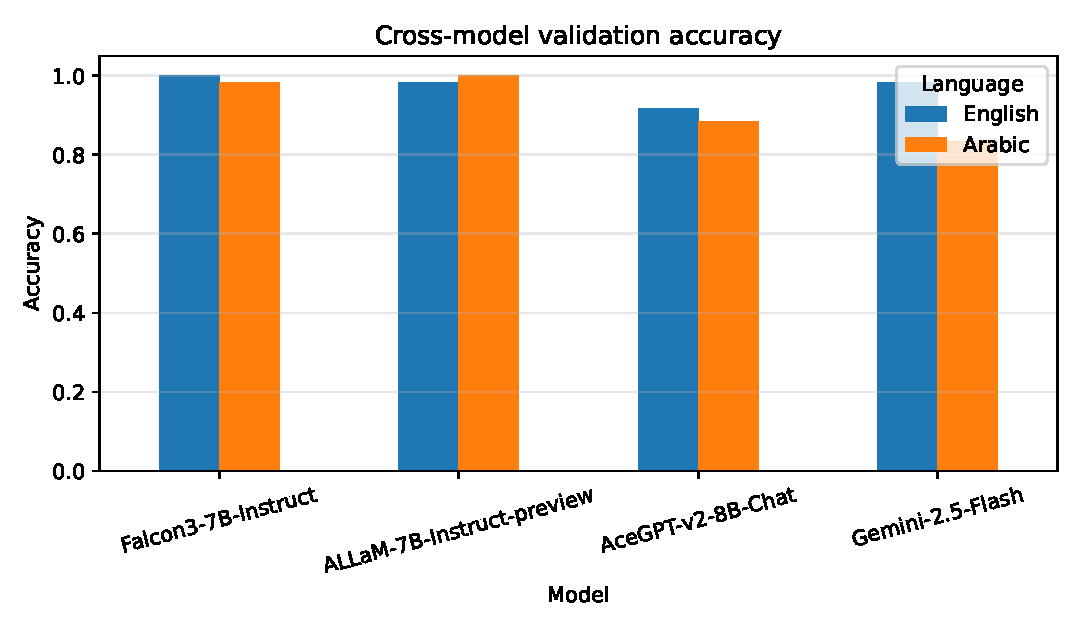
\includegraphics[width=\linewidth]{../figures/cross_model_accuracy.pdf}\caption{Cross-model accuracy by language.}\label{fig:acc}\end{figure}
\begin{figure}[H]\centering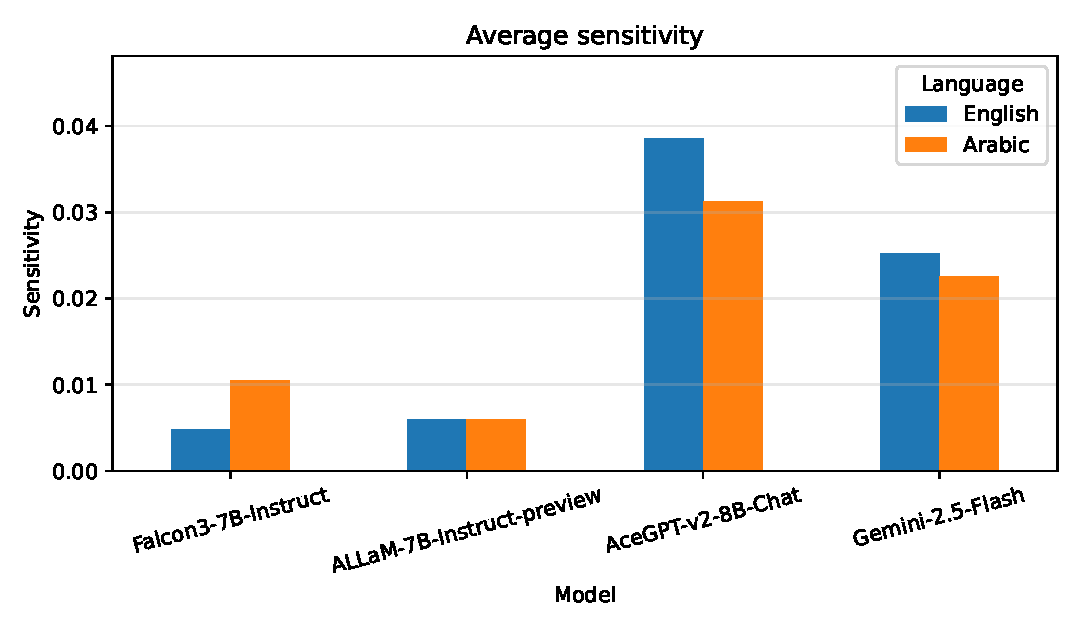
\includegraphics[width=\linewidth]{../figures/cross_model_sensitivity.pdf}\caption{Average sensitivity by model and language.}\label{fig:sens}\end{figure}
\begin{figure}[H]\centering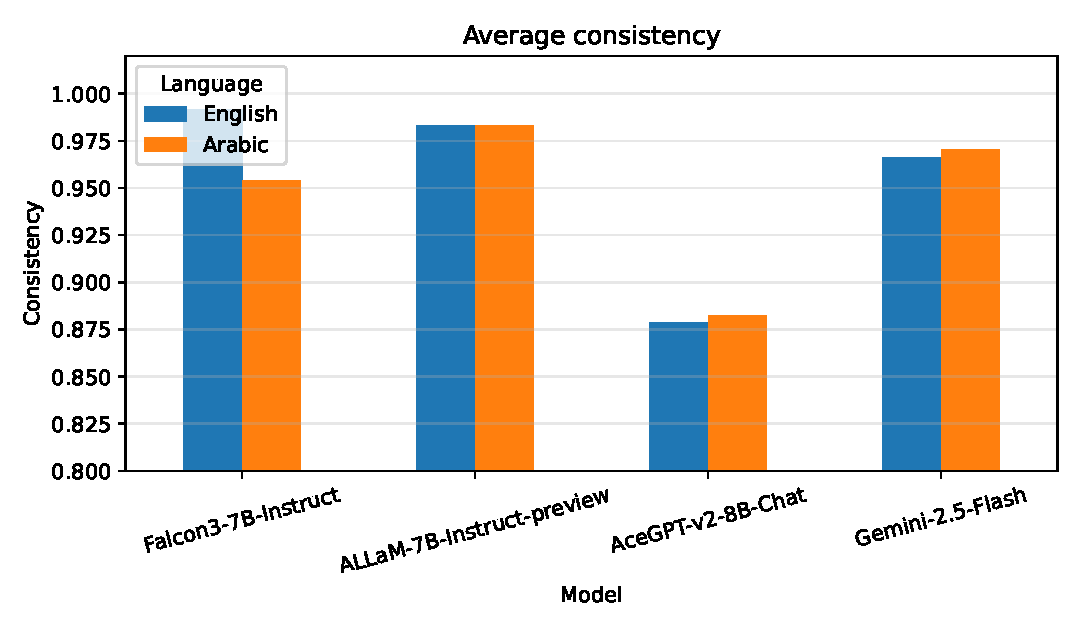
\includegraphics[width=\linewidth]{../figures/cross_model_consistency.pdf}\caption{Average consistency by model and language.}\label{fig:cons}\end{figure}
\subsection{Class-Level Results}
\begin{table*}[t]\centering\caption{Class-level accuracy. Each cell is majority-vote accuracy for 10 samples.}\label{tab:classlevel}\resizebox{\textwidth}{!}{\begin{tabular}{llrrrr}\toprule Language & Label & Falcon3 & ALLaM & AceGPT & Gemini\\\midrule English & NUMBER & 1.0 & 1.0 & 1.0 & 1.0\\ English & LOCATION & 1.0 & 1.0 & 1.0 & 1.0\\ English & PERSON & 1.0 & 1.0 & 1.0 & 1.0\\ English & DESCRIPTION & 1.0 & 1.0 & 1.0 & 1.0\\ English & ENTITY & 1.0 & 0.9 & 0.5 & 1.0\\ English & ABBREVIATION & 1.0 & 1.0 & 1.0 & 0.9\\ Arabic & NUMBER & 1.0 & 1.0 & 1.0 & 1.0\\ Arabic & LOCATION & 1.0 & 1.0 & 1.0 & 1.0\\ Arabic & PERSON & 0.9 & 1.0 & 1.0 & 1.0\\ Arabic & DESCRIPTION & 1.0 & 1.0 & 1.0 & 1.0\\ Arabic & ENTITY & 1.0 & 1.0 & 0.3 & 1.0\\ Arabic & ABBREVIATION & 1.0 & 1.0 & 1.0 & 0.0\\\bottomrule\end{tabular}}\end{table*}

\begin{figure}[H]\centering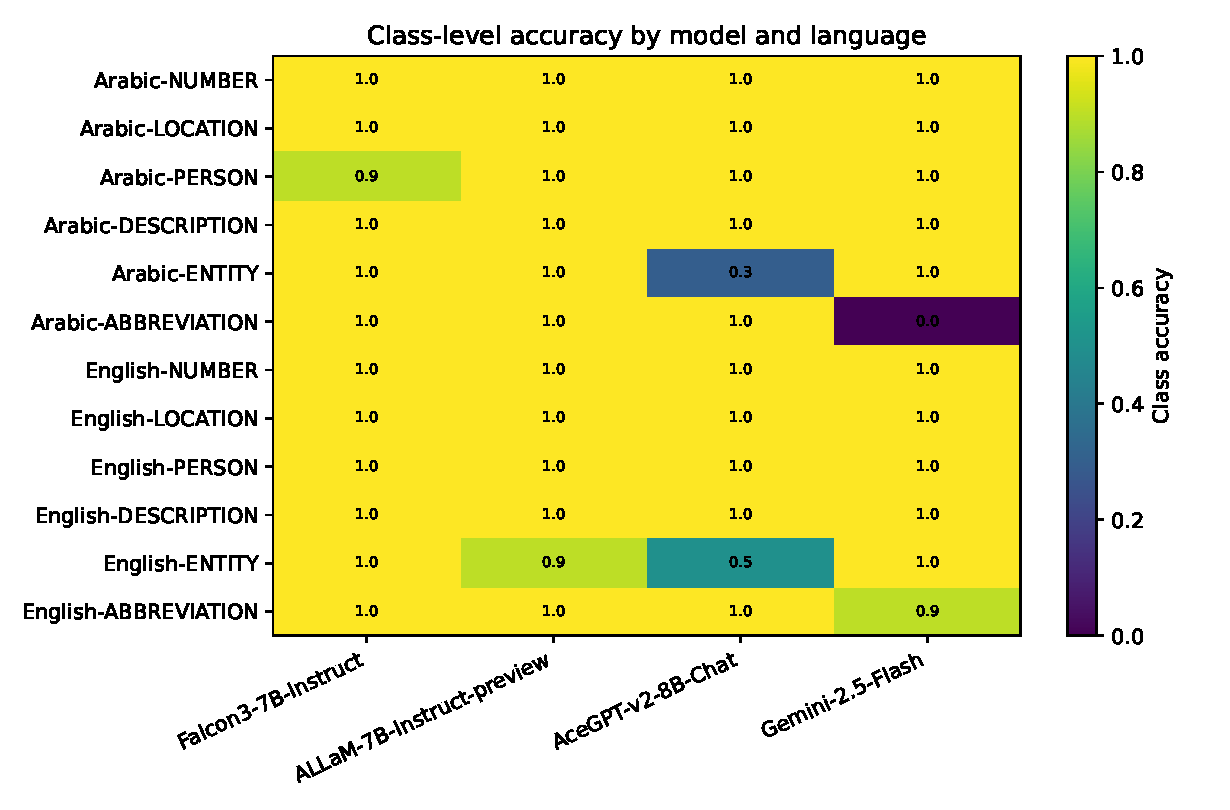
\includegraphics[width=\linewidth]{../figures/class_level_accuracy_heatmap.pdf}\caption{Class-level accuracy heatmap. Gemini's Arabic ABBREVIATION failure is visible as the lowest cell.}\label{fig:classheat}\end{figure}
\subsection{Statistical Tests and Confidence Intervals}
\begin{table}[H]\centering\caption{Bootstrap 95\% confidence intervals for validation accuracy.}\label{tab:ci}\resizebox{\linewidth}{!}{\begin{tabular}{llrrr}\toprule Model & Lang. & Acc. & CI Low & CI High\\\midrule Falcon3 & English & 1.0000 & 1.0000 & 1.0000\\ Falcon3 & Arabic & 0.9833 & 0.9500 & 1.0000\\ ALLaM & English & 0.9833 & 0.9500 & 1.0000\\ ALLaM & Arabic & 1.0000 & 1.0000 & 1.0000\\ AceGPT & English & 0.9167 & 0.8500 & 0.9667\\ AceGPT & Arabic & 0.8833 & 0.8000 & 0.9500\\ Gemini & English & 0.9833 & 0.9500 & 1.0000\\ Gemini & Arabic & 0.8333 & 0.7333 & 0.9167\\\bottomrule\end{tabular}}\end{table}

\begin{figure}[H]\centering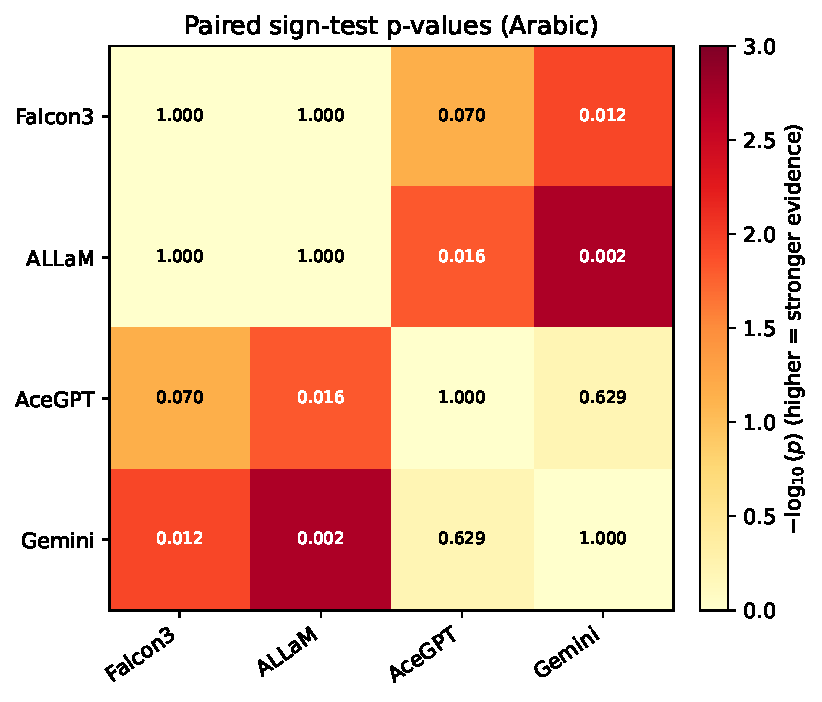
\includegraphics[width=\linewidth]{../figures/pairwise_pvalue_heatmap_arabic.pdf}\caption{Arabic paired sign-test p-values for model comparisons. Values show p; color intensity shows $-\log_{10}(p)$.}\label{fig:pvalar}\end{figure}
\begin{figure}[H]\centering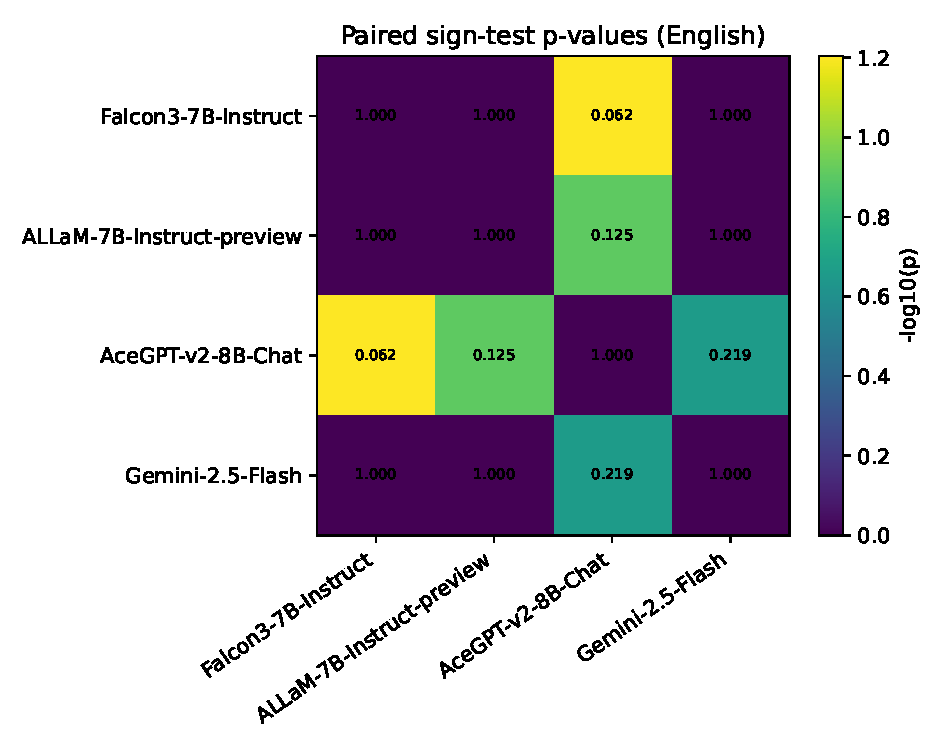
\includegraphics[width=\linewidth]{../figures/pairwise_pvalue_heatmap_english.pdf}\caption{English paired sign-test p-values for model comparisons.}\label{fig:pvalen}\end{figure}
\section{Discussion / Analysis}
The pilot progression supports RQ1 and RQ2: prompt design strongly affected the Falcon3 results. Adding definitions helped both languages; adding few-shot examples stabilized Arabic; and adding a targeted DESCRIPTION/ENTITY rule fixed most of the earlier Arabic DESCRIPTION errors. This suggests that some apparent model weakness was actually label-boundary ambiguity that could be reduced through prompt design.

RQ3 is partly supported. The frozen prompt generalized well to Falcon3 and ALLaM, and it remained competitive on AceGPT. Gemini showed high English accuracy but lower Arabic accuracy under compact variants. The Arabic Gemini errors were not random: all ten Arabic ABBREVIATION samples were predicted as DESCRIPTION. This suggests that Arabic questions equivalent to ``What does the abbreviation ... mean?'' were interpreted as asking for meaning or explanation rather than for an acronym-expansion category. This is valuable because the sensitivity score alone was low: the model was stable, but stably wrong for one class.

The results therefore show why accuracy, sensitivity, consistency, and error analysis should be interpreted together. Low sensitivity is useful only when the stable behavior is correct. A model can be robust across prompt variants while still mapping one language-specific cue to the wrong class.
\section{Conclusion}
This study evaluated prompt design for English-Arabic question-type classification. The best prompt combined definitions, few-shot examples, and a targeted DESCRIPTION/ENTITY disambiguation rule. On unseen validation, this design reached near-perfect results for Falcon3 and ALLaM and strong results for AceGPT. Gemini 2.5 Flash achieved 0.9833 English accuracy and 0.8333 Arabic accuracy under eight compact variants, with Arabic ABBREVIATION as the dominant failure mode. The main conclusion is that targeted prompt clarification can reduce bilingual label confusion, but closed-model compact prompting still requires language-specific error analysis.
\section*{Limitations}
The dataset is small, balanced, and manually constructed, so it cannot represent all real English-Arabic question distributions. Each class has only 10 examples per language in validation. The prompt was refined through prior error analysis, so broader validation is needed. Arabic dialects were not evaluated. The Gemini compact variants were intentionally short to prevent output truncation, which may have reduced Arabic abbreviation guidance. Hugging Face models were run with 4-bit quantization, which can differ from full-precision inference. Finally, API models can change over time.
\section*{Ethics Statement}
This project uses a small educational dataset and does not require private or sensitive user data. The main ethical risk is overclaiming from a small benchmark. To reduce this risk, we report limitations, raw predictions, class-level errors, confidence intervals, and exact prompts. API keys are not stored in the repository and should be supplied only through environment variables or notebook secrets.
\section*{Code and Data Availability}
All code, prompts, result CSV files, figures, and reproducibility materials are included in this repository package.
\section*{Acknowledgements}
This project was completed for the Prompt Engineering course at the Mediterranean Institute of Technology. We thank Professor Abdeldjalil Labed for the project guidelines and evaluation framework. We also acknowledge the open-source model developers, the Hugging Face ecosystem, and the Google Gemini API ecosystem.
\begin{thebibliography}{99}
\bibitem{ailem2024robustness} Melissa Ailem et al. 2024. Examining the robustness of LLM evaluation to the distributional assumptions of benchmarks. arXiv:2404.16966.
\bibitem{brown2020language} Tom B. Brown et al. 2020. Language models are few-shot learners. \textit{NeurIPS}.
\bibitem{chen2024calls} Lingjiao Chen et al. 2024. Are more LLM calls all you need? Toward scaling laws of compound inference systems. arXiv:2403.02419.
\bibitem{errica2025wrong} Federico Errica et al. 2025. What did I do wrong? Quantifying LLMs' sensitivity and consistency to prompt engineering. arXiv:2406.12334v4.
\bibitem{geng2024confidence} Jiahui Geng et al. 2024. A survey of confidence estimation and calibration in large language models. \textit{NAACL}.
\bibitem{hendrycks2021mmlu} Dan Hendrycks et al. 2021. Measuring massive multitask language understanding. \textit{ICLR}.
\bibitem{huang2023ceval} Yuzhen Huang et al. 2023. C-Eval: A multi-level multi-discipline Chinese evaluation suite for foundation models. \textit{NeurIPS}.
\bibitem{huang2024acegpt} Huang Huang et al. 2024. AceGPT, localizing large language models in Arabic. \textit{NAACL}.
\bibitem{humain2025allam} HUMAIN. 2025. ALLaM-7B-Instruct-preview model card. Hugging Face.
\bibitem{kojima2022large} Takeshi Kojima et al. 2022. Large language models are zero-shot reasoners. \textit{NeurIPS}.
\bibitem{li2002learning} Xin Li and Dan Roth. 2002. Learning question classifiers. \textit{COLING}.
\bibitem{liang2023helm} Percy Liang et al. 2023. Holistic evaluation of language models. \textit{TMLR}.
\bibitem{lu2022fantastically} Yao Lu et al. 2022. Fantastically ordered prompts and where to find them. \textit{ACL}.
\bibitem{mccoy2023embers} R. Thomas McCoy et al. 2023. Embers of autoregression: Understanding large language models through the problem they are trained to solve. arXiv:2309.13638.
\bibitem{ouyang2022training} Long Ouyang et al. 2022. Training language models to follow instructions with human feedback. \textit{NeurIPS}.
\bibitem{sahoo2024survey} Pranab Sahoo et al. 2024. A systematic survey of prompt engineering in large language models. arXiv:2402.07927.
\bibitem{sclar2024quantifying} Melanie Sclar et al. 2024. Quantifying language models' sensitivity to spurious features in prompt design. \textit{ICLR}.
\bibitem{tii2025falcon3} Technology Innovation Institute. 2025. Falcon3-7B-Instruct model card. Hugging Face.
\bibitem{voorhees2000building} Ellen M. Voorhees and Dawn M. Tice. 2000. Building a question answering test collection. \textit{SIGIR}.
\bibitem{wang2023selfconsistency} Xuezhi Wang et al. 2023. Self-consistency improves chain of thought reasoning in language models. \textit{ICLR}.
\bibitem{wei2022chain} Jason Wei et al. 2022. Chain-of-thought prompting elicits reasoning in large language models. \textit{NeurIPS}.
\bibitem{white2023prompt} Jules White et al. 2023. A prompt pattern catalog to enhance prompt engineering with ChatGPT. arXiv:2302.11382.
\bibitem{zhao2021calibrate} Zihao Zhao et al. 2021. Calibrate before use: Improving few-shot performance of language models. \textit{ICML}.
\end{thebibliography}
\appendix
\onecolumn
\section{Final Frozen Prompt Strategy}
The final prompt structure was: task statement, six allowed labels, label definitions, one example per label, DESCRIPTION/ENTITY disambiguation rule, and exact-label-only output constraint. Complete prompt files are included under \texttt{prompts/}.
\begin{lstlisting}[caption={Final English prompt skeleton.}]
You are a question-type classifier.
Classify the question into exactly one of these labels:
NUMBER, LOCATION, PERSON, DESCRIPTION, ENTITY, ABBREVIATION.
Definitions: NUMBER = number/date/quantity; LOCATION = place; PERSON = human; DESCRIPTION = explanation/meaning/function/process; ENTITY = specific non-person/non-location thing; ABBREVIATION = acronym or expansion.
Examples: How many planets are in the Solar System? -> NUMBER; Where is the Eiffel Tower located? -> LOCATION; Who wrote Hamlet? -> PERSON; What is photosynthesis? -> DESCRIPTION; What planet is known as the Red Planet? -> ENTITY; What does CPU stand for? -> ABBREVIATION.
Rule: Choose DESCRIPTION for explanation, meaning, definition, function, purpose, use, or process. Choose ENTITY for a specific object, animal, planet, language, currency, device, material, gas, software, element, metal, or instrument.
Question: {question}
Output exactly one label only.
\end{lstlisting}
\begin{lstlisting}[caption={Compact Gemini prompt skeleton.}]
Strictly classify this question by expected answer type.
Labels: NUMBER, LOCATION, PERSON, DESCRIPTION, ENTITY, ABBREVIATION.
Rule: DESCRIPTION for explanation/meaning/function/use/process; ENTITY for a specific thing.
Question: {question}
Label:
\end{lstlisting}
\section{Dataset and Result Files}
The full English and Arabic validation CSV files are available in the repository under \texttt{data/}. Raw predictions are under \texttt{results/raw_predictions/}; evaluated metrics are under \texttt{results/metrics/}. Representative examples include a bicycle-wheel count question (NUMBER), a Statue of Liberty location question (LOCATION), and an Arabic ATM-abbreviation question (ABBREVIATION).
\section{Statistics Code Used}
\begin{lstlisting}[language=Python,caption={Bootstrap accuracy confidence interval code used.}]
import numpy as np

def bootstrap_accuracy_ci(correct, n_boot=10000, seed=42):
    rng = np.random.default_rng(seed)
    correct = np.asarray(correct, dtype=float)
    n = len(correct)
    idx = rng.integers(0, n, size=(n_boot, n))
    values = correct[idx].mean(axis=1)
    return np.percentile(values, [2.5, 97.5])
\end{lstlisting}
\end{document}
